% !TeX spellcheck = cs_CZ
%{\tikzset{external/prefix={tikz/CES/}}
% \tikzset{external/figure name/.add={ch02_}{}}
%---------------------------------------------------------------------------------------------------
% file Basic_MCU_Arch.tex
%---------------------------------------------------------------------------------------------------
\lstset{ %
  language={[x86masm]Assembler},         % choose the language of the code
  inputencoding=latin1,
  extendedchars=true,
  showspaces=false,                      % show spaces everywhere adding particluar undescores, it  
                                         % overrides 
                                         % “showstringspaces”
  showstringspaces=false,                % underline spaces within strings only
  basicstyle=\footnotesize\ttfamily,     % the size of the fonts that are used for the code
%  backgroundcolor=\color{White},        % choose the background color. You must add  
                                         % \usepackage{color}
  breaklines=true,                       % sets automatic line breaking
  breakatwhitespace=true,                % sets if automatic breaks should only happen at whitespace
  showspaces=false,                      % show spaces adding particular underscores
  showstringspaces=true,                 % underline spaces within strings
  showtabs=true,                         % show tabs within strings adding particular underscores
  frame=none,                            % adds a frame around the code - none, single
  tabsize=2,                             % sets default tabsize to 2 spaces
  captionpos=b,                          % sets the caption-position to bottom
  numbers=left,                          % where to put the line-numbers -none, left, right
  numberstyle=\tiny\color{lstnumcolor},  % the size of the fonts that are used for the line-numbers
  numbersep=5pt,                         % how far te line-number are from the code
  stepnumber=1,                          % the step between two line-numbers. If it's 1 each line
                                         % will be numbered
  xleftmargin=3em,                       % adjust left margin
  commentstyle=\color{help}\textit,      % comment style
  keywordstyle=\color{keyword}\textbf,   % keyword style
  morekeywords={ADDC, ASHR, SUBB,CLR,    % if you want to add more keywords to the set
    MAC,  MULS, DIVS, BSET, BCLR, BCPL, 
    BAND, BOR,  BXOR, BCMP, TRL,  EX,  BMOV,
    JCC,  BCC,  DJNZ, RETI, JSR,  CSP, LDR},
  literate= %
    {á}{{\'a}}1  {é}{{\'e}}1     {í}{{\'i}}1   {ó}{{\'o}}1   {ú}{{\'u}}1
    {Á}{{\'A}}1  {É}{{\'E}}1     {Í}{{\'I}}1   {Ó}{{\'O}}1   {Ú}{{\'U}}1
    {à}{{\`a}}1  {è}{{\`e}}1     {ì}{{\`i}}1   {ò}{{\`o}}1   {ù}{{\`u}}1
    {À}{{\`A}}1  {È}{{\'E}}1     {Ì}{{\`I}}1   {Ò}{{\`O}}1   {Ù}{{\`U}}1
    {ä}{{\"a}}1  {ë}{{\"e}}1     {ï}{{\"i}}1   {ö}{{\"o}}1   {ü}{{\"u}}1
    {Ä}{{\"A}}1  {Ë}{{\"E}}1     {Ï}{{\"I}}1   {Ö}{{\"O}}1   {Ü}{{\"U}}1
    {â}{{\^a}}1  {ê}{{\^e}}1     {î}{{\^i}}1   {ô}{{\^o}}1   {û}{{\^u}}1
    {Â}{{\^A}}1  {Ê}{{\^E}}1     {Î}{{\^I}}1   {Ô}{{\^O}}1   {Û}{{\^U}}1
    {œ}{{\oe}}1  {Œ}{{\OE}}1     {æ}{{\ae}}1   {Æ}{{\AE}}1   {ß}{{\ss}}1
    {ç}{{\c c}}1 {Ç}{{\c C}}1    {ø}{{\o}}1    {å}{{\r a}}1  {Å}{{\r A}}1
    {€}{{\EUR}}1 {£}{{\pounds}}1 {ř}{{\v{r}}}1 {ž}{{\v{z}}}1 {č}{{\v{c}}}1
    {ě}{{\v{e}}}1
}
%================== Kapitola: Základy mikroprocesorové techniky====================================
%\setchaptertoc
\chapter{Historie mikroprocesorové techniky}
\minitoc
    \subsection{Vývoj mikroprogramových řadičů: od mainframu EDSAC k moderním 
                 mikroprocesorům}\hypertarget{MIT:sec_003}
      Na princip funkce mikrořadiče řízeného pomocí mikroprogramů, jenž byl popsaný v kapitole 
      \ref{ces:IchapIVsecIIssecI}, se můžeme dívat jako na zobecnění idey programování počítačů 
      pomocí instrukcí uložených v operační paměti. V samých počátcích vývoje výpočetní techniky, 
      konkrétně u takzvané nulté generace (zhruba do roku 1947) a první generace (cca roky 1946 až 
      1958) počítačů, se totiž algoritmy nevyjadřovaly pomocí instrukcí tvořících ucelené programy, 
      které by byly uloženy do paměti. Namísto toho byl algoritmus „zadrátován“ (obr. 
      \ref{MIT:fig_eniac}) takovým způsobem, že se pomocí vodičů umístěných většinou na spínacích 
      panelech vzájemně propojovaly jednotlivé moduly počítače – sčítačky, pracovní registry, 
      řadiče paměti, vstupní prvky atd. Navíc se u některých specializovaných počítačů používaných 
      za druhé světové války pro luštění šifer nedal algoritmus vůbec měnit – počítač stále 
      prováděl stejné výpočty, ovšem s různými daty. Tato konstrukce počítačů odpovídala dobové 
      technologii, které se používala především v telefonních ústřednách s ručním přepojováním 
      hovorů, semaforech nebo například pro ovládání výtahů.
      
      \begin{figure}[ht!]   %\ref{MIT:fig_eniac}
        \centering
        \includegraphics[width=0.9\linewidth]{eniac.jpg}
        \caption{Způsob programování elektronického počítače \Eniac (\emph{Electronic Numerical 
                 Integrator And Computer}) pomocí vzájemného propojování jednotlivých modulů 
                 přepojováním kabelů mezi jednotlivými funkčními moduly. Kredit: Columbia 
                 university}
        \label{MIT:fig_eniac}
      \end{figure}
      
      \subsubsection{Von Neumannova architektura programovatelného počítače}
        Ovšem již v polovině čtyřicátých let minulého století přišel \wikiNeumann s převratnou 
        myšlenkou – libovolný algoritmus nemusí být přímo „zadrátován“ v počítači, ale může být 
        zapsán ve formě programu složeného ze sekvence instrukcí, které mohou být uloženy v paměti 
        počítače naprosto stejným způsobem, jako zpracovávaná data; viz též dnes již klasické von 
        Neumannovo dílo \wikiEDVAC vydané v roce 1945. Právě díky této myšlence vznikly první 
        skutečné procesory s instrukčními sadami, děrné štítky se začaly používat mj. i pro uložení 
        programů a navíc se otevřela cesta k dalšímu zobecnění: programy začaly být asi o deset let 
        později vytvářeny ve vyšších programovacích jazycích, přičemž překlad prováděl jiný program 
        (algoritmus) nazývaný překladač (dnes bereme překladače jako zcela běžnou věc, ale idea, že 
        překladač je sám o sobě taktéž algoritmem, byla v době její implementace chápána jako malá 
        revoluce). Toto dvojí zobecnění práce univerzálního programovatelného počítače nebylo 
        dodnes překonáno a je na něm založena i moderní výpočetní technika a informatika.
        
        Architektura počítačů navržená John von Neumannem byla založena na \emph{centrální 
        procesorové jednotce} rozdělené na \emph{aritme\-ticko-logickou jednotku} a 
        \emph{řadič}, 
        který na základě instrukcí čtených z operační paměti řídil všechny další moduly počítače 
        (vstupně-výstupní zařízení, aritmeticko-logickou jednotku, operační paměť). Nikde ovšem 
        nebylo přesně specifikováno, jakým způsobem má být řadič, jakožto „mozek“ počítače, 
        implementován. V prvních mainframech založených na myšlence Johna von Neumanna se tedy 
        uplatňovaly obvodové řadiče. Tyto řadiče byly dostatečně rychlé a nevyžadovaly ke své 
        činnosti prakticky žádné paměťové prvky (většinou jen čítač či posuvný registr), ovšem 
        přinášely i některé nevýhody. Jednou z poměrně závažných nevýhod byla velká složitost 
        obvodového řadiče v případě, že se používala komplexnější instrukční sada (\texttt{CISC}). 
        Poněkud paradoxně se právě složité instrukční sady začaly v padesátých letech minulého 
        století stále více používat, zejména na mainframech druhé generace. A právě tehdy se začala 
        prakticky realizovat myšlenka \emph{mikroprogramování}.
      
      \subsubsection{EDSAC – první počítač se skutečným mikroprogramovým řadičem}
        Myšlenka mikroprogramování vznikla již v roce 1951, kdy ji ve svých článcích představil sir 
        \wikiEWilkes (titul sir získal Wilkes právě za svoji dlouholetou práci v oboru 
        \texttt{IT}). Idea mikroprogramování spočívala v zobecnění konstrukce centrální procesorové 
        jednotky (\texttt{CPU}) takovým způsobem, že strojové instrukce byly rozkládány na sekvenci 
        řídicích signálů pomocí mikroprogramu uloženého v paměti typu \texttt{ROM} s velmi rychlou 
        dobou přístupu. Vzhledem ke stavu technologie v roce 1951 samozřejmě V. Wilkes nemohl 
        použít klasický čip s \texttt{ROM}, v němž jsou bity trvale zaznamenány s použitím 
        poslední, zákazníkem definované masky při výrobě čipu. Namísto toho Wilkes navrhoval použít 
        matici navzájem kolmých vodičů, v níž by byla bitová jednička „zaznamenána“ pomocí diody 
        spojující jeden vodorovný a jeden svislý vodič (vodivou kovovou spojku nelze použít, 
        protože by se do matice nepřímo zapsaly i falešné jedničky).
        
        \begin{figure}[ht!]   %\ref{MIT:fig_edsac}
          \centering
          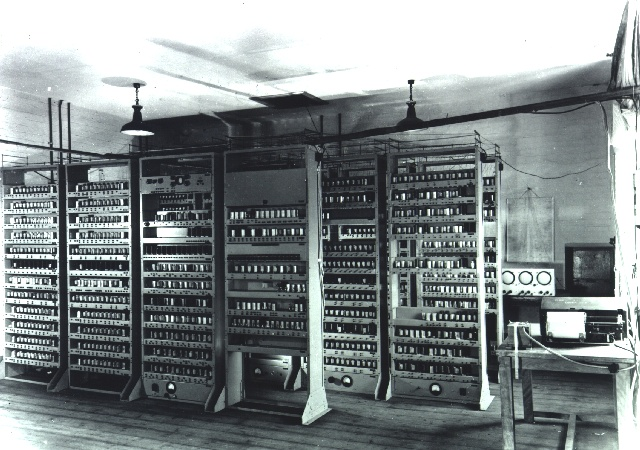
\includegraphics[width=0.95\linewidth]{EDSAC.jpg}
          \caption{\wikiEDSAC (Electronic Delay Storage Automatic Calculator) byl britský počítač z 
                   poloviny 20. století. Tento počítač, inspirovaný John Von Neumannovým dokumentem 
                   First Draft of a Report on the EDVAC, sestavil Maurice Wilkers a jeho tým na 
                   Univerzitě v Cambridgi v Anglii. EDSAC byl první v praxi využitý počítač 
                   pracující s uloženým programem. Kredit: Wikipedia, Root.cz}
          \label{MIT:fig_edsac}
        \end{figure}
        
        Na zpočátku pouze teoretickou práci M. V. Wilkese o několik let později navázali William 
        Renwick a \wikiWheeler, kteří v roce 1957 sestrojili první skutečný počítač založený na 
        mikroprogramovém procesoru. Vzhledem k tomu, že diodová matice navržená Wilkesem by byla 
        příliš rozměrná pro počítač s velkou instrukční sadou (diodami jsou zde samozřejmě myšleny 
        diskrétní elektronické součástky, i když se v roce 1957 již pomalu schylovalo k výrobě 
        prvních prototypů integrovaných obvodů), použili W. Renwick a D. Wheeler namísto diod 
        feritovou paměť, což bylo ve svém důsledku velmi zajímavé, protože se obsah této paměti dal 
        přeprogramovat a tím pádem bylo možné i měnit instrukční sadu počítače. První prototyp 
        tohoto stroje byl nazván \texttt{EDSAC 1½} a používal pro uložení mikroinstrukcí feritovou 
        paměť s maticí o velmi malých rozměrech 6×8 feritových jader – tento počítač ovšem 
        neobsahoval celou instrukční sadu. Finální podoba počítače z roku 1958, jež nesla název 
        \texttt{EDSAC 2}, měla již paměťovou matici o rozměrech 32×32 feritových jader, což již 
        umožnilo implementaci plnohodnotné instrukční sady za použití mikrokódů.
    
%} % tikzset
%---------------------------------------------------------------------------------------------------
\printbibliography[title={Seznam literatury}, heading=subbibliography]
\addcontentsline{toc}{section}{Seznam literatury}